\section{Numbers and Sets}

\subsection{Sets}

\Def[Set(Class)]{.}
\begin{Sym}
    $\in, \subseteq, \subset, [A,B](\cap), \wedge(\cup)$
\end{Sym}

\subsection{Mappings. Cardinality}

\begin{Def}[Function]
    $\forall a\in \mathcal{M},\exists \text{only one} \phi(a)\in \mathcal{N}$.
    \begin{align*}
        \text{image: } & \{\phi(a): a\in \mathcal{M}\}  \\
        \text{preimage: } & \{a: \exists \phi(a) \in \text{image}(\phi)\}   \\
        \text{surjective(onto): } & \forall y \in \text{image}(\phi), \exists a \rightarrow \phi(a)=y   \\
        \text{injective(one-one): } & \phi(a) = \phi(b) \rightarrow a = b   \\
        \text{inverse: } & \phi^{-1}\phi=I_\mathcal{M}; \phi\phi^{-1}=I_\mathcal{N}
    \end{align*}
\end{Def}

\begin{Them}[Bernstein]。
    \[
        |\mathcal{M}|=|\mathcal{N}|:= \exists \text{bijective } \phi: \mathcal{M}\rightarrow \mathcal{N}
    \]
    We say $\mathcal{M}$ and $\mathcal{N}$ are equipotent or have same cardinality.
\end{Them}

\subsection{The Number Sequence}

\begin{Axm}[Peano]
    \begin{align*}
        &1 \text{ is a natural number.}  \\
        &\forall \text{natural number } a \text{ has a definite successor } a^+ \in N   \\
        &\forall a\in N, a^+ \neq 1 \\
        &\forall a,b\in N,a^+=b^+ \rightarrow a=b    \\
        &X\subseteq N. 1 \in X, \forall a \in X, a^+\in X \rightarrow X=N  
    \end{align*}
    The five axiom is called the principle of mathematical induction.
\end{Axm}

Sum of two numbers.

\begin{Def}[Addition $+$]
    \[
        +(x,y):=
        \begin{cases}
            \forall x, x+1=x^+  \\
            \forall x,y, x+y^+=(x+y)^+
        \end{cases}
    \]
\end{Def}

\begin{Prop}[Addition]
    \begin{align*}
        \text{Associative}:& (a+b)+c=a+(b+c) \\
        \text{Commutative}:& a+b=b+a \\
        \text{Cancellative}:& a+b=a+c \rightarrow b=c
    \end{align*}
\end{Prop}

\begin{Def}[Product $\cdot$]
    \[
        \cdot(x,y):=
        \begin{cases}
            \forall x, x\cdot 1=x   \\
            \forall x,y, x\cdot y^+=x\cdot y+x
        \end{cases}
    \]
\end{Def}

\begin{Prop}[Product]
    \begin{align*}
        \text{Associative}:&(a\cdot b)\cdot c=a\cdot(b\cdot c)  \\
        \text{Commutative}:&a\cdot b=b\cdot a   \\
        \text{Cancellative}:& a\cdot b=a\cdot c\rightarrow b=c
    \end{align*}    
\end{Prop}

\begin{Prop}[Addition and Product, Distributive]
    \[
        a\cdot(b+c)=a\cdot b+a\cdot c
    \]
\end{Prop}

\begin{Def}[Order, Greater, Less]
    $a>b:=\exists u \in N, a=b+u.$     
\end{Def}

\begin{Prop}[Order]
    \begin{align*}
        &\forall a,b, \text{only one relation } a<b, a=b, a>b \text{ hold.}   \\
        &a<b \wedge b<c \rightarrow a<c  \\
        &a<b \rightarrow a+c<b+c \\
        &a<b \rightarrow ac < bc
    \end{align*}   
\end{Prop}

\begin{Them}
    Every nonempty set of natural numbers contains a least number. 
\end{Them}

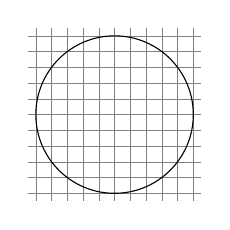
\begin{tikzpicture}
    \draw[step=0.2cm,gray, very thin] (-1.1,-1.1) grid (1.1,1.1);
    \draw (0,0) circle[radius=1];
\end{tikzpicture}

\subsection{Finite and Countable (Denumerable) Sets}

\subsection{Partitions}